The main requirement of the FAR-EDGE CPS Data Model presented the in previous section is to provide full support within the architecture for digital continuity to the \textit{Open API for Virtualization}(see Figure~\ref{fig:architectureSimulation}. 
In other words, the data model has been designed with the goal of : 
\begin{enumerate}
\item providing tools to fully describe simulation models to be imported and executed by FAR-EDGE compliant simulators and,
\item streamlining the definition of complex synchronization processes to be carried out by the Real-to-Digital Synchronization (R2DS) component. 
\end{enumerate}

The Real-to-Digital Synchronization can be defined as the process of continuously updating the CPS digital twins stored in the \textit{Model Repository}, following the evolution of the shop floor. 
Clearly, having reliable models is especially important in simulation. 
In fact, machines along their life cycle are subject to aging, straining, and reconfiguration processes, which might affect their behavior and performance; in this case the simulation outcomes to drift apart substantially from reality and, therefore, result useless. 
In order to be able to make informed decisions it is of paramount importance to detect divergences in the model \textit{automatically} (because given the number of  potentials CPS in the shop it can be unfeasible for this activity to be done manually) and \textit{continuously} (simulation can be sensitive to even small parameter changes), and to adapt parameters and scenarios accordingly. 

The core of the R2DS grounds in the processing of data gathered at shop floor level. 
It is worth noticing that this is a general approach, based on data processing, which enables not only the tracking of CPS models parameters but it also unlocks scenarios where, for instance, digital twins can be enriched with inferred pieces of information that cannot be directly measured from the field. 
For illustration purposes, let's imagine the case in which a digital twin is extended with the results of a machine learning algorithm designed for predictive maintenance~\cite{daily2017predictive}. 
Ideally, this algorithm is no different from those that track parameters to avoid drift and its outcome can be stored as property of the related digital twin  to be used from the simulation to schedule the most suitable time to perform the maintenance of the real machine.  

In order to achieve the most general and adaptable system possible, the simulation system has been designed and built in such a way as to be agnostic of the particular data collection and analysis system provided by the "analytics" domain of the architecture. In particular, as mentioned when the model was presented, third-party tools may require different and/or proprietary models and languages in order to be used. Therefore, while fully supporting the reference implementation of the FAR-EDGE architecture, it was decided to introduce the concept of synchronization directly within the simulation model. The \textit{Synchronization Model} (SM), a particular \textit{artifact} (and as such independent from the platform), has been defined specifically for the implementation of the synchronization process at the level of the single digital twin.
This is because each digital twin might require a different data processing  to be synchronized with its real counterpart. 

Figure~\ref{fig:sm-diagram} presents one of the sub-models of the core model presented in Section~\ref{sec:model}. In particular, the synchronization model can be seen alongside more commonly used simulation artifacts (kinematic model, logic model, geometry). 


\begin{figure}
	\centering
	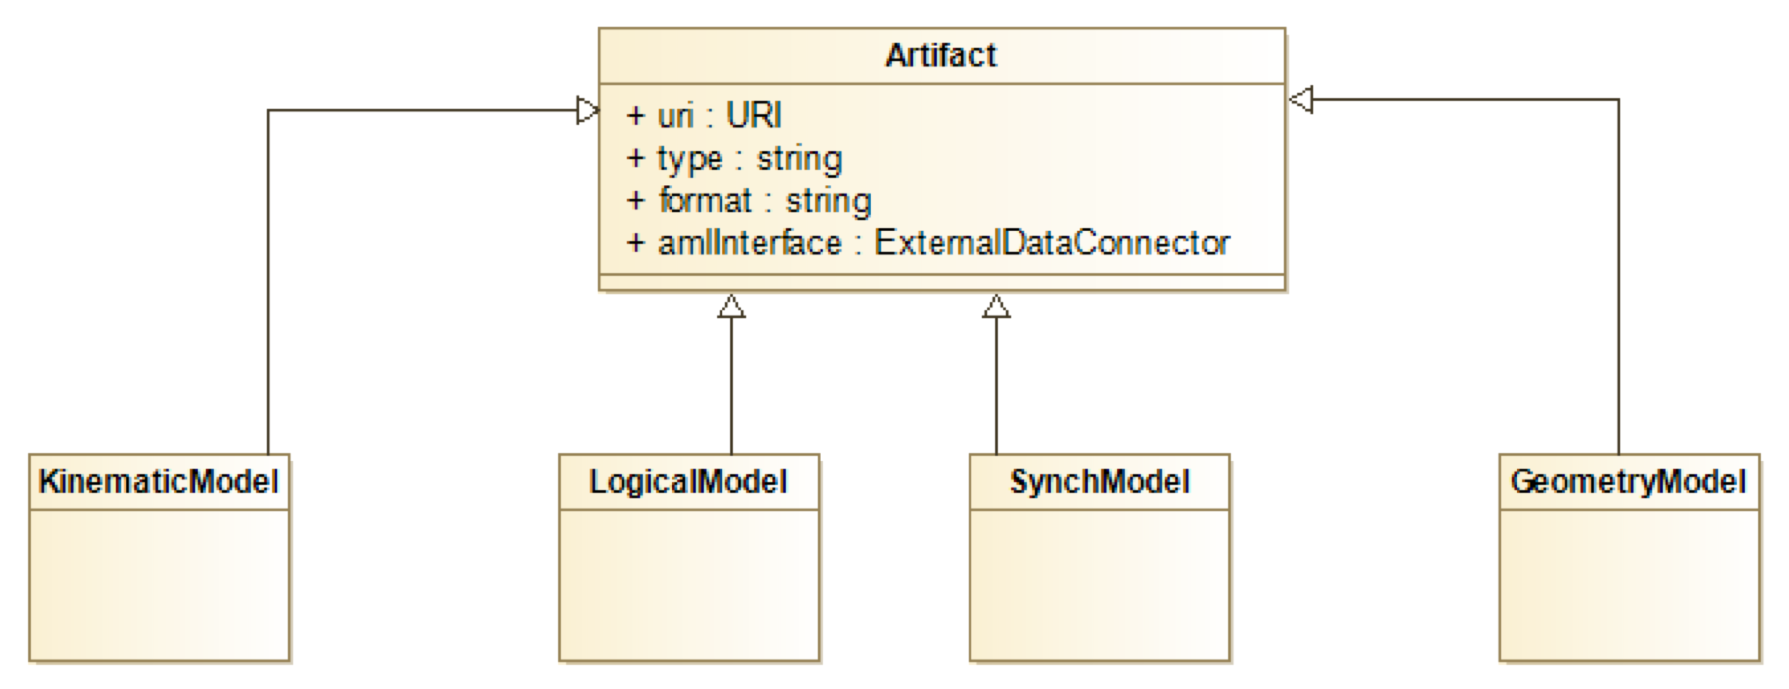
\includegraphics[width=0.9\linewidth]{images/sm-artifact.png}
	\caption{Diagram representing the main Artifact-derived concepts}
	\label{fig:sm-diagram}
\end{figure}

Synchronization Models describe the way data from the field must be processed to update the model attributes or to estimate indirect values and create new attributes. 
A synchronization model contains an algorithmic description of how to process data from machine sensors at shop floor level in order to generate updates that continuously serve to keep the digital twin digital in sync with the related CPS. 
This description can therefore be instantiated in different ways depending on the technological choices that underlie the implementation of the platform. 
The solution adopted in the project is to implement the synchronization model in the form of a simulation asset, that is a binary file containing executable code and to associate it with the representation of a CPS within the data model. The synchronization model, therefore, in order to perform its duty, must be compiled, installed and managed within a suitable execution environment, which can provide through an API the abstractions necessary to process data coming from the production environment in a distributed way.  


Specific components will be in charge of managing the life cycle of Synchronization Models, which includes: 
\begin{enumerate}
\item \textbf{Execution notification}- depending on the synchronization scenario the system can be notified about the presence of a new CPS and the SM is executed against streams of field data (if the CPS is reachable and producing data), or SM is scheduled to run periodically, say for instance, once a day over historical data. If the CPS has no corresponding item in the list of active digital twins a suitable structure is created using meta-data associated with the data stream. In this case however, only limited virtualization and synchronization operations can be performed.
\item \textbf{Model fetching}- if the digital twin has a SM registered, it is looked up and retrieved from a suitable database where it is persisted. 
\item \textbf{Execution}- the SM is run exploiting \textit{FAR-EDGE Open API for Analytics} and\textit{ Synchronization Services}.
\item \textbf{Digital twin updating}- the SM generates attribute values for the related digital twin. These values are used to update the digital twin, which the model refers to.
\item \textbf{Model dismissal}- once the dismissal condition is verified (as, for instance, the CPS is not connected or the synchronization process ended) the SM is dismissed and the \textit{Synchronization Services} sub-system is notified.
\end{enumerate}



\begin{figure}
	\centering
	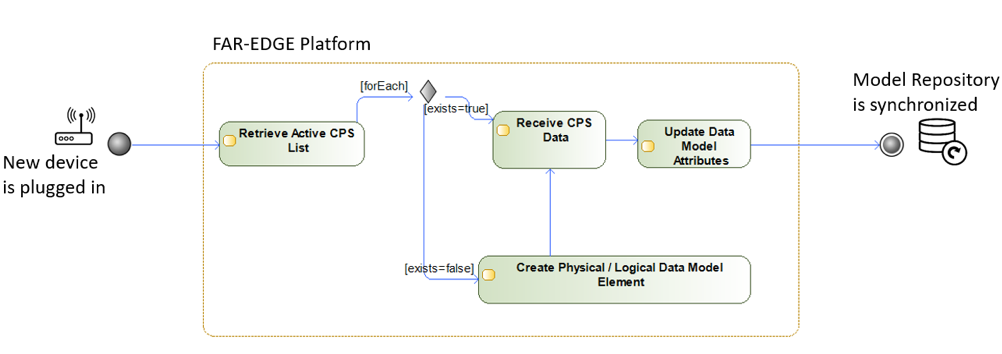
\includegraphics[width=\linewidth]{images/sm-scenario2}
	\caption{Synchronization process}
	\label{fig:sm-scenario}
\end{figure}

Figure~\ref{fig:sm-scenario} presents by means of an activity diagram the main steps to achieve digital-to-real synchronization. Figure~\ref{fig:r2ds}, instead, describes the same reference scenario from an architectural point of view. In this scenario a CPS is plugged into the FAR-EDGE platform, is presence is noticed by the FAR-EDGE monitoring application, the R2DS Component is notified and the CPS can start to generate data which are spawned via the \textit{Data Routing and Preprocessing Component} of the architecture. 
If a SM associated with the CPS digital twin in the model repository is available, it will be retrieved and executed on the Synchronization Services, which in turn rely on the Edge Analytics Engine provided by the \textit{Analytics} domain. 
In this scenario, the SM processes the input data flow and generates a new stream, containing for each time interval updates for the corresponding digital twin. 
%The R2DS component is in charge of performing the model update process. 

It is worth restating at this point that the algorithm implemented within a SM it is not constrained to the generation of attribute updates for digital twins, but it is general. In this way, for instance, the same infrastructure and the overall process can be used to enrich the CPS definition with new pieces of information. 

\begin{figure}
	\centering
	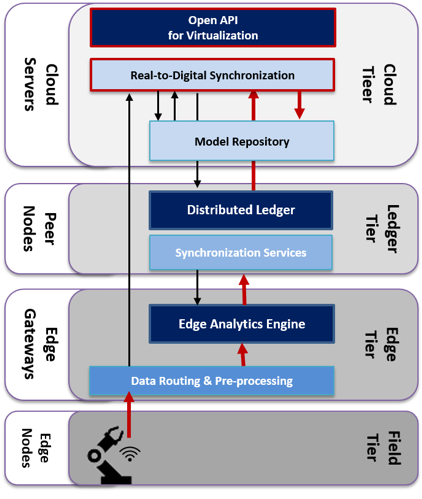
\includegraphics[width=0.7\linewidth]{images/R2DS}
	\caption{Synchronization process - Architectural view}
	\label{fig:r2ds}
\end{figure}


